\documentclass[11pt,letterpaper]{report}
\usepackage{amssymb,amsfonts,color,graphicx,amsmath,enumerate}
\usepackage{amsthm}

\newcommand{\naturals}{\mathbb{N}}
\newcommand{\integers}{\mathbb{Z}}
\newcommand{\complex}{\mathbb{C}}
\newcommand{\reals}{\mathbb{R}}
\newcommand{\mcal}[1]{\mathcal{#1}}
\newcommand{\rationals}{\mathbb{Q}}
\newcommand{\field}{\mathbb{F}}
\newcommand{\Var}{\text{Var}}
\newcommand{\ind}{\mathbbm{1}}
\newcommand{\Cov}{\text{Cov}}

\newenvironment{solution}
{\begin{proof}[Solution]}
{\end{proof}}

\voffset=-3cm
\hoffset=-2.25cm
\textheight=24cm
\textwidth=17.25cm
\addtolength{\jot}{8pt}
\linespread{1.3}

\begin{document}
\begin{center}
{\bf \Large Math 180B - A Fermat-Type Equation and Square-Triangle Numbers}
\vspace{0.2cm}
\hrule
\end{center}

\begin{enumerate}
	\item Show that the equation $x^2+y^2 = 9z+3$ has no integral solution.

	\item Consider a right triangle, the lengths of whose sides are integers. Prove that the area cannot be a perfect square.

	\item Here is a descent argument showing the irrationality of $\sqrt{2}$.
	\begin{itemize}
		\item Assume $\sqrt{2}$ is rational and write $\sqrt{2} = 1+\frac{p}{q}$ where $p<q$.
		\item Then $2q^2 = q^2 + 2pq+p^2 \implies p^2 = q(q-2p)\implies \frac{p}{q} = \frac{q-2p}{p}$.
		\item But now $\sqrt{2} = 1+\frac{q-2p}{p}$ has fractional part with denominator $p$ smaller than $q$. Repeating the argument, we obtain an argument by descent.
	\end{itemize}
	Generalize the argument to prove that $\sqrt{n}$ is irrational whenever $n\in \naturals$ is not a perfect square. \textit{Hint: write $\sqrt{n} = m+\frac{p}{q}$ where $m$ is the integer part of $\sqrt{n}$.}

	\item Show that the equation $x^2-dy^2 = -1$ has no solutions if $d\equiv 3\pmod{4}$.

	\item A number $n$ is called a pentagonal number if $n$ pebbles can be arranged in the shape of a filled in pentagon. The first four pentagonal numbers are 1, 5, 12, and 22, as illustrated in Figure 1. You should visualize each pentagon as sitting inside the next larger pentagon. The $n$-th pentagonal number is formed using an outer pentagon whose sides have $n$ pebbles.
	\begin{figure}[h]
		\centering
			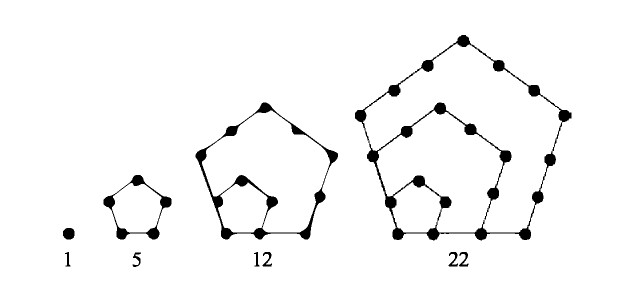
\includegraphics[scale=.6]{pent.PNG}
			\caption{The First Four Pentagonal Numbers}	
	\end{figure}
	\begin{enumerate}[(a)]
		\item Find a formula for the $n$-th pentagonal number.
		\item Recall that square-triangular numbers correspond to solutions to the equation $x^2-2y^2=1$. Find a similar equation for square-pentagonal numbers.
	\end{enumerate}
\end{enumerate}



\end{document}